\documentclass{beamer}
\mode<presentation>
\usepackage{algorithm,amssymb,amsmath,amsthm,bbm,color,epstopdf,float,geometry,graphicx,hyperref,listings,mathrsfs,mathtools,multirow,subcaption,textgreek,xcolor}
\usepackage[noend]{algpseudocode}
\usepackage[flushleft]{threeparttable}
\usepackage[shortlabels]{enumitem}

% Create Background Pic
%\usepackage{tikz}
%\definecolor{bottomcolour}{rgb}{0.32,0.3,0.38}
%\definecolor{topcolour}{rgb}{0.08,0.08,0.16}
%\setbeamertemplate{background canvas}{%
%	\begin{tikzpicture}[remember picture,overlay]
%	\shade[top color=topcolour,bottom color=bottomcolour]
%(current page.north west) rectangle (current page.south east);
%	\end{tikzpicture}%     
%}


%=======================================================
% Set page number
\setbeamertemplate{footline}[page number]

%=======================================================
%\usetheme{Boadilla}
\setbeamerfont{title}{size=\fontsize{18pt}{18pt}\selectfont} % bold font: \bfseries
\setbeamerfont{author}{size=\fontsize{20pt}{20pt}\selectfont}
\setbeamerfont{institute}{size=\fontsize{13pt}{13pt}\selectfont}
%\setbeamercolor{itemize item}{fg=red}

%================================================
%Set font color
\definecolor{mygray1}{rgb}{0.7421875,0.7421875,0.7421875}
\definecolor{mygray2}{gray}{0.6}
\definecolor{mygray3}{rgb}{0.55, 0.52, 0.54}
\definecolor{mybrown1}{rgb}{0.28, 0.24, 0.2}
\definecolor{myred}{rgb}{0.68, 0.09, 0.13}
\definecolor{myginger}{rgb}{0.69, 0.4, 0.0}
\definecolor{myblue1}{rgb}{0.0, 0.2, 0.6}
\definecolor{myblue2}{rgb}{0.38, 0.51, 0.71}
\definecolor{myblue3}{rgb}{0.2,0.2,0.7}
\definecolor{mygreen}{rgb}{0.42, 0.56, 0.14}
\definecolor{myviolet}{rgb}{0.54, 0.17, 0.89}


\newcommand{\highlightA}[1]{\colorbox{myblue3!50!}{$\displaystyle #1$}}
\newcommand{\highlightB}[1]{\colorbox{myred!50!}{$\displaystyle #1$}}
\newcommand{\highlightC}[1]{\colorbox{mygreen!50!}{$\displaystyle #1$}}
%================================================
% set picture source
\usepackage[absolute,overlay]{textpos}

\setbeamercolor{framesource}{fg=gray}
\setbeamerfont{framesource}{size=\tiny}
\newcommand{\source}[1]{\begin{textblock*}{4cm}(8.7cm,8.6cm)
\begin{beamercolorbox}[ht=0.5cm,right]{framesource}
\usebeamerfont{framesource}\usebeamercolor[fg]{framesource} Source: {#1}
\end{beamercolorbox}
\end{textblock*}}

\setbeamercolor{frametitle}{fg=white,bg=black}


%================================================
% url color
\renewcommand\UrlFont{\color{myblue3}}
%================================================

\newtheorem{Thm}{{\bf Theorem}}


% Make first page
\makeatletter
\setbeamertemplate{navigation symbols}{}
\title[AMSC 663 Advanced Scientific Computing I]{\Large  
Multi-fidelity Monte Carlo}
%\subtitle[short version]{}
%\date{}
\author[Jiaxing Liang]{\large Dr. Jiaxing Liang (Rice University)\\
Dr. Matthias Heinkenschloss (Rice University)}
\vspace{-5cm}
%\institute[UMD]{University of Maryland, College Park}
%\usetheme{Pittsburgh}
%\usecolortheme{owl}

%======Footline=================================================
%\makeatother
%\setbeamertemplate{footline}
%{
%	\leavevmode%
%	\hbox{%
%%		\begin{beamercolorbox}[wd=.4\paperwidth,ht=2.25ex,dp=1ex,center]{author in head/foot}%
%%			\usebeamerfont{author in head/foot}\insertshortauthor
%%		\end{beamercolorbox}%
%		\begin{beamercolorbox}[wd=\paperwidth,ht=2.25ex,dp=1ex,leftskip=4.3cm,rightskip=.3cm plus1fil]{topcolour}
%			\usebeamerfont{title in head/foot}\insertshorttitle\hfill%\hspace*{3em}
%			\insertframenumber{} / \inserttotalframenumber\hspace*{1ex}
%	\end{beamercolorbox}}%
%\begin{beamercolorbox}[wd=.1\paperwidth,ht=2.25ex,dp=1ex,right,rightskip=2ex]{page number in head/foot}%
%	%            \usebeamerfont{title in head/foot}\insertshorttitle\hspace*{3em}
%	\insertframenumber{} / \inserttotalframenumber
%\end{beamercolorbox}%    
%	\vskip0pt%
%}

%=======================================================
\begin{document}
\frame{\titlepage }


% %------------------------------------------------------------
% \begin{frame}[t]
%     \frametitle{Multi-fidelity Monte Carlo}

%     \begin{itemize}[leftmargin=5pt] 
%             \item[$\triangleright$] Multi-fidelity Monte Carlo (MFMC): 

%             a variance reduction technique used in computational simulations to efficiently estimate quantities of interest by combining multiple models of varying accuracy and computational cost.

%             \item[$\triangleright$] Idea:
            
%             Instead of relying solely on high-fidelity (accurate but expensive) simulations, MFMC strategically integrates low-fidelity (less accurate but cheaper) models to reduce computational cost while maintaining accuracy. It optimally balances the number of simulations at different fidelity levels to minimize computational budget given an error.

%             MFMC is particularly useful in scenarios where high-fidelity simulations are prohibitively expensive but necessary for accuracy, making it a powerful tool in computational science and engineering.
    

    

%     \end{itemize}


% \end{frame}

% %------------------------------------------------------------
% \begin{frame}[t]
%     \frametitle{Multi-fidelity Monte Carlo}

%     \begin{itemize}[leftmargin=5pt] 
%      \vspace{3mm}
%         \item[$\triangleright$] How It Works:
%         \begin{itemize}[leftmargin=15pt]
%             \item[$\circ$] Multiple Fidelity Levels: It leverages models of different fidelities—e.g., simplified physics-based models, surrogate models, or coarse-grid simulations.
            
%             \item[$\circ$] Control Variate Approach: The low-fidelity models act as control variates to correct and improve estimates from the expensive high-fidelity model.

%             \item[$\circ$] Optimal Sampling Strategy: MFMC determines the optimal number of simulations to run at each fidelity level to achieve the best trade-off between accuracy and cost.
%         \end{itemize}

%     \end{itemize}


% \end{frame}





% \begin{frame}[t]{stellar}
% \frametitle{Necessary conditions -- $t_f$ free}
% {\footnotesize
% \begin{itemize}[leftmargin=5pt] 
%     \item[] 
%     \begin{align*}
%     \text{Lagrangian} \quad &J = \varphi + \nu_b^Tb + \nu_p^T p + \nu_s^T s+\\ 
%     &\int_{t_0}^{t_f}  L + \lambda^t \left[f - \dot{x}\right] 
%     \;dt\\
%         \text{Hamiltonian} \quad &H(t, x, u, \lambda) = L(t, x, u) + \lambda(t)^T f(t, x, u),\\
%          \text{Control} \quad &u^* = \operatorname*{argmin}_{u\in \mathcal{U}}\, H(t, x^*, u,\lambda^*),\quad \forall t\in[t_0, t_f],\\
%         \text{State} \quad &\dot{x} = \frac{\partial H}{\partial \lambda},\\
%         \text{Adjoint equation} \quad &\dot{\lambda} = -\frac{\partial H}{\partial x},\\
%         \text{T ransversality cond} \quad &\lambda (t_f) = 
%     \end{align*}
% \end{itemize}
% }	
% \end{frame}


%}
%=================================================
% Imagine two positive nuclei in my hand, two forces acting on them: nuclear force (attract them) and coulub force(push them aways), when at big distance, nuclei repel each other, when find ways to conquer the coulomb force barrier, two neulei get closed to each other and merge into one heavier neulcei. mass defect release energy. example: sun. 

%Tokamak: russian word--toroidal chamber with magnetic coils. see below two figures. Inject fuel gas into the chamber and heat with microwave, becomes fluid of particles -- called plasma, high temperature, vibrate fast, high speed easy to overcome coulum repulsion and get closed to each other, and collide to produce energy.
%=================================================
% Q: the distance of repel & attract?


% %------------------------------------------------------------
% \begin{frame}[t]
% \frametitle{Plasma Confinement}
% %		\begin{columns}
% %			\begin{column}{0.8\textwidth}

% During fusion, the hot plasma tends to expand, to prevent it from contacting the reactor wall, it must be confined. 

% \vspace{4mm}
% {\fontsize{13}{13}\selectfont \textcolor{myblue3}{\bf Question: How to maintain confinement of hot plasma?} }

% \vspace{2mm}
% \begin{itemize} [leftmargin=5pt] 
% \vspace{-3mm}
% \item[$\triangleright$] Since plasmas are conductive and magnetically tractable -- use a \textcolor{myred}{\bf magnetic field}  generated by currents in  external coils around the fusion reactor.
% \vspace{1.8mm}

% %When heated to fusion temperatures, the electrons in atoms disassociate, resulting in a fluid of nuclei and electrons known as a plasma. Unlike electrically neutral atoms, a plasma is electrically conductive, and can, therefore, be manipulated by electrical or magnetic fields.
% \item[$\triangleright$] Our project focuses on studying the \textcolor{myred}{\bf impact of variations in current} on the physical properties of the confinement field.


% \begin{equation*}
% \hspace{-11mm}
% \text{Variations}
% \left\{ \begin{array}{l}
% \text{Power supply}\\ [3pt]
% \text{Temperature fluctuations}\\ [3pt]
% \text{Material impurities in the conduction wire}
% \end{array}\right.
% \end{equation*}


% \item []
% %\begin{figure}[H]	
% %	\centering
% %	\begin{tabular}{cc}
% %		\begin{subfigure}{0.45\textwidth}
% %			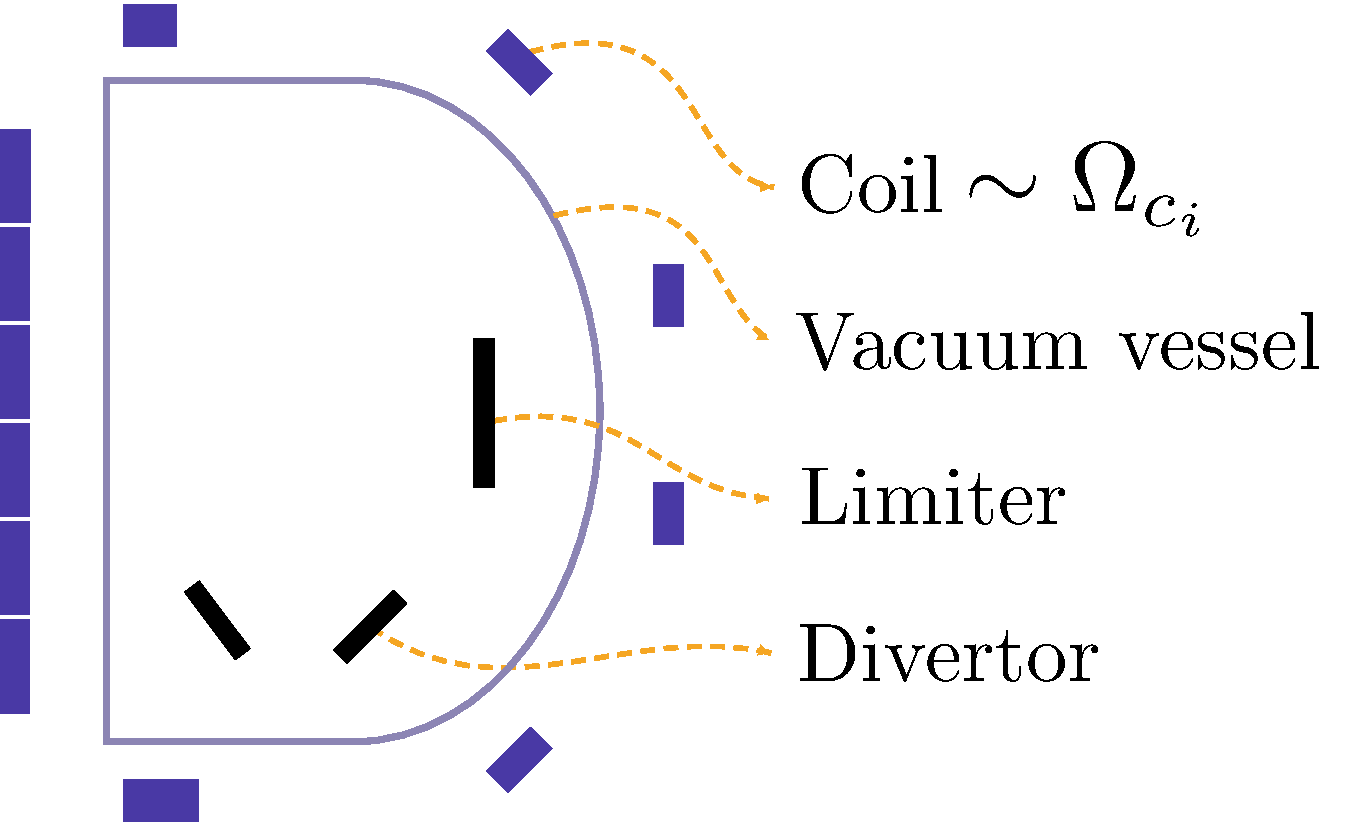
\includegraphics[height=0.55\linewidth]{../../../Project/Plot/BasicConfig}
% %%			\caption*{Divertor configuration}
% %		\end{subfigure}
% %		&
% %		\begin{subfigure}{0.45\textwidth}
% %			\includegraphics[height=0.55\linewidth]{../PictureFolder/PlasmaImage}
% %			\source{https://en.wikipedia.org/wiki/Mega{\_}Ampere{\_}Spherical{\_}Tokamak}
% %%			\caption*{Limiter configuration}
% %		\end{subfigure}
% %	\end{tabular} 
% %\end{figure}
% \end{itemize}
% \end{frame}



%=================================================
% We impose the bottom two conditions. if x is 0, then the equation becomes singular, so the first condition avoid singularity in the equation, and the second equaiton shows the decay of function at infinity, and ensure the uniqueness of the solution.
%=================================================

% %------------------------------------------------------------
% \begin{frame}[t]
%     \frametitle{Uncertainty Quantification (UQ)}
%     \begin{itemize}[leftmargin=5pt]
%         \item[$\triangleright$] \textcolor{myblue3}{\bf Source of uncertainty:} {\footnotesize Investigate the impact of \textcolor{myblue3}{uncertainties in the current intensities} on the confinement properties of a plasma.}
        
%         \item[$\triangleright$] \textcolor{myred}{\bf Baseline current intensities:} 
%         \[
%         \footnotesize
%         \begin{array}{lll}
%         I_1: -1.40\times 10^6\text{A} &I_5: -9.00\times 10^6\text{A} &I_9:  -6.43\times 10^6\text{A} \\
%         I_2: -9.50\times 10^6\text{A} &I_6: 3.56\times 10^6\text{A}  & I_{10}:  -4.82\times 10^6\text{A} \\
%         I_3: -2.04\times 10^7\text{A} &I_7:  5.47\times 10^6\text{A}  &I_{11}:  -7.50\times 10^6\text{A} \\
%         I_4: -2.04\times 10^7\text{A} &I_8: -2.27\times 10^6\text{A} &I_{12}:  1.72\times 10^7\text{A} 
%         \end{array}
%         \]
%         \item[$\triangleright$] \textcolor{myblue3}{\bf Uncertianty Quantification:} {\footnotesize Variations in the baseline current intensities. Each current in the array is considered to be a parameter, so we have 12-dimensional parameter space.}
        
        
%         \item[$\triangleright$] \textcolor{myblue3}{\bf Currents uniformly distributed:} 

%         {\footnotesize
%         \textcolor{mygray3}{$\tau$: perturbation level ($\tau= 1\%$ \& $2\%$). \quad $I_k$: current intensity in the $k$-th coil.}
        

%         \begin{itemize}[leftmargin=15pt]   
%             \item[$\circ$] Joint density function: $\displaystyle
%              \pi \left(\boldsymbol{\omega}\right)=\prod_{k=1}^{d} \pi_k\left(\omega_{k}\right)=\prod_{k=1}^{d} \frac{1}{2\tau |I_k|}$.
%             \item[$\circ$] 12-d parameter space: $\displaystyle W := \prod_{k=1}^{d}\left[I_k-\tau|I_k|,I_k+\tau|I_k|\right]$.
%         \end{itemize}
%         \par}
%     \end{itemize}
% \end{frame}	
%=================================================
% here I list an example of an array of currents, each current in the array is considered to be a parameter, so we have 12 dimensional parameter space, and if we use 1%...., we will use MC method to handle the uncertainty.
%=================================================











% %------------------------------------------------------------
% \begin{frame}[t]
%     \frametitle{Random space: from infinite to finite dimension}
    
%     \begin{itemize}[leftmargin=5pt] 
%             \item[$\triangleright$] \textcolor{myblue3}{\bf Finite dimensional noise assumption:}  
            
%         {\footnotesize
%         To solve the problem numerically, we need to reduce the infinite-dimensional space to a finite-dimensional space. This is often achieved via a certain type of decomposition which can approximate the target random process with desired accuracy.

%         Eg. Karhunen-Loève type expansion. 
%         }

%         \item[$\triangleright$] \textcolor{myblue3}{\bf Result:} 
        
%         {\footnotesize
%         The random inputs can be characterized by $d$ random variables.

%         \begin{equation*}
%             \left\{ \begin{array}{ll}
%             \mathcal{L}(t, x) = f(t, x, \omega) = f(t, x, Y^1(\omega), \cdots, Y^{d}(\omega)) & t \in D\\
%             \mathcal{B}(t, x) = g(t)& t \in \partial D
%             \end{array}\right.
%         \end{equation*}
%         where $\{Y^k\}_{k=1}^{d}$ are real-valued random variables with zero mean and unit variance. Each is mutually independent with probability density $\pi_k: \Gamma^k\rightarrow \mathbb{R}^+$ with image $\Gamma^k = Y^k(\omega)$ are bounded intervals in $\mathbb{R}$ for all $k$. Let $\boldsymbol{y}=(Y^1, \cdots Y^{d})$. The joint density and support of $\boldsymbol{y}$ are 
%         \begin{align*}
%              \pi \left(\boldsymbol{y}\right)=\prod_{k=1}^{d} \pi_k(Y^{k}), \quad W = \prod_{k=1}^{d} \Gamma^k.
%         \end{align*}

        
%         We assume this equation admits a unique solution $x^{d} = x^{d}(t, \omega) = x^d(t, Y^1(\omega), \cdots, Y^d(\omega))$. 
%         }
%     \end{itemize}
% \end{frame}

% %------------------------------------------------------------
% \begin{frame}[t]
%     \frametitle{Random space: from infinite to finite dimension}
    
%     \begin{itemize}[leftmargin=5pt] 

%         \item[$\triangleright$]
        
%         {\footnotesize
%         This allows to rewrite the problem as $(d+d_D)$ dimensional differential equation:

%         \begin{equation*}
%             \left\{ \begin{array}{ll}
%             \mathcal{L}(t, x) = f(t, x, \boldsymbol{y}) & (\boldsymbol{y}, t) \in W\times D\\
%             \mathcal{B}(t, x) = g(t)& (\boldsymbol{y}, t) \in W\times \partial D
%             \end{array}\right.
%         \end{equation*}
%         where $d$ and $d_D$ are the dimension of random space $W$ and physical space $D$ respectively.

%         Our goal is to approximate the function $x^d = x^d(t, \boldsymbol{y})$ for any $\boldsymbol{y}\in W$ and $t\in D$.
%         }
%     \end{itemize}
% \end{frame}



% %------------------------------------------------------------
% \begin{frame}[t]
%     \frametitle{Physical space: from infinite to finite dimension}
    
%     \begin{itemize}[leftmargin=5pt] 

%         \item[$\triangleright$]
        
%         {\footnotesize
%         Next, we approximate the problem in a finite element subspace.

%         \vspace{2mm}
%         Let $\widehat{\pi}$ be a finite element operator $\widehat{\pi}: Z\rightarrow Z_h$ with the optimality condition
%         \[
%         \|\varphi - \widehat{\pi}_h \varphi\|_Z\le C_{\widehat{\pi}} \min_{v\in Z_h}\|\varphi - v\|_Z, \quad \forall \varphi\in Z,
%         \]
%         where $C_{\widehat{\pi}}$ is independent of mesh size $h$.

%         \vspace{3mm}
%         Let $Z_h\subset Z$ be a standard FE space of dimension $N_h$. It contains continuous piecewise polynomials defined on regular triangulations $\mathcal{T}_h$ that have a maximum mesh parameter $h>0$. $Z_h$ has the following deterministic approximate property:

%         For a given function $\varphi \in Z$,
%         \[
%         \min_{v\in Z_h} \|\varphi - v\|_Z \le C(s;\varphi) h^s,
%         \]
%         where $s$ is a positive integer determined by the smoothness of $\varphi$ and the degree of the approximating finite element subspace.

%         $C(s;\varphi)$ is independent of $h$.
%         }
%     \end{itemize}
% \end{frame}







% %------------------------------------------------------------
% \begin{frame}[t]
%     \frametitle{Interpolation error}
    
%     \begin{itemize}[leftmargin=5pt] 
%     % \item[$\triangleright$] a 'function space' is a collection of functions with similar properties, where each function in the space is considered as an element, allowing operations like addition and scalar multiplication to be performed on them, often with restrictions based on the desired properties (like continuity or differentiability) of the functions within that space
    
%     \item[$\triangleright$] \textcolor{myblue3}{For functions in the space $F_d^k$}
%     \[
%     F_d^k = \left\{ f: [-1, 1]^d\rightarrow \mathbb{R}\big |\quad \partial^{|\boldsymbol{m}|}f \text{ continuous if } m_i\le k\; \forall i\right\}
%     \]
%     $\partial^{|\boldsymbol{m}|}$: d-variate partial derivative of order $|\boldsymbol{m}|$.
% \item[$\triangleright$]  For our problem, the fr\'echet derivative of x with respect to $\omega$ is twice continuously differentiable
    
%     \end{itemize}

    
%     \fbox{%
%     \parbox{1.01\textwidth}{
%     \textcolor{myblue3}{\bf Theorem:} {\footnotesize Interpolation error bound in $L_\infty$ norm
%     \vspace{-2mm}
%     \[\|(I_d-\mathscr{S})(f)\|_\infty = \mathscr{O}\left(N^{-k}\cdot \vert \log N\vert ^{(k+2)(d-1) +1}\right)\vspace{-2mm}\]
%     $N$: \# of collocation nodes, $d$: dimension, $k$: measure of smoothness of $f$ wrt $\boldsymbol{\xi}$.}}}

% \end{frame}


% %------------------------------------------------------------
% \begin{frame}[t]
%     \frametitle{Stochastic collocation}
%     {\footnotesize
%     \begin{itemize}[leftmargin=5pt] 
%             \item[$\triangleright$]  For our problem, to estimate trajectory, 
            
%             $x: D\rightarrow \mathbb{R}$, $Z = W_{1, \infty}(D)$. 

%             The fr\'echet derivative of x with respect to $\omega$ is twice continuously differentiable.
        
        
%     \end{itemize}
%     }
% \end{frame}


% %------------------------------------------------------------
% \begin{frame}[t]
%     \frametitle{Stochastic collocation}
%     {\footnotesize
%     \begin{itemize}[leftmargin=5pt] 
%             \item[$\triangleright$]  Sparse grid nodes: Chebyshev Gauss-Lobatto nodes $X^i = \{x_1^i, \cdots, x_{m_i}^i\}, i\in \mathbb{N}$.
%             {\footnotesize
%             \begin{itemize}[leftmargin=15pt]
%             \item[$\circ$] Nodes are nested $X^i\subset X^{i+1}$, include the end points of the interval.
%             \item[$\circ$] 
%             \begin{align*}
%                 m_i &= \left\{ \begin{array}{ll}
%                 1  &\text{if } i = 1,\\
%                 2^{i-1}+1 &\text{if } i > 1.
%                 \end{array}\right.
%                 \\
%                 X^i_j &= \left\{ \begin{array}{ll}
%                 \frac{1}{2}\left(-\cos\left(\frac{j-1}{m_i-1}\pi\right)+1\right)  &\text{for } j = 1, \cdots, m_i, \text{ if } m_i>1, \\
%                 \frac{1}{2} &\text{for } j=1, \text{ if } m_i = 1.
%                 \end{array}\right.
%             \end{align*}
%             \item[$\circ$] These are the roots of the Chebyshev polynomials of the second kind with degree $m_i$.
%             \end{itemize}
%             }
        
        
%     \end{itemize}
%     }
% \end{frame}




% %------------------------------------------------------------
% \begin{frame}[t]
%     \frametitle{Uncertainty quantification: Drag and Lift coefficient}
    
%     \begin{itemize}[leftmargin=5pt] 
    
%     \item[$\triangleright$] \textcolor{myblue3}{\bf Lift and drag forces:} {\footnotesize $\text{Lift: } L = \frac{1}{2}C_L \rho V^2S, \quad \text{Drag: } D=\frac{1}{2}C_D \rho V^2S $,}
    
%     \begin{align*}
%         \text{Atmospheric density:} \quad &\rho(y) = 1.225\times 10^9e^{-0.14y}\;\;[kg/m^3] \\
%         \text{Altitude:} \quad &y \;\; [m]\\
%         \text{Total velocity of vehicle:} \quad &V\;\; [m/s]\\
%         \text{Dynamic pressure:} \quad &\frac{1}{2} \rho V^2 \;\; [Pa]  \\
%         \text{Wing area:} \quad &S = 6\times 10^{-6} \;\; [m^2] \\
%         \text{Lift coefficient:} \quad &C_L = -0.04 + 0.8\alpha \\
%         \text{Drag coefficient:} \quad &C_D = 0.012 - 0.01\alpha + 0.6\alpha^2 \\
%         \text{Angle of attack:} \quad &\alpha \;\; [^\circ]
%     \end{align*}
    
%     % \item[$\triangleright$] \textcolor{myblue3}{\bf Drag:} {\footnotesize.}
    
%     % \item[$\triangleright$] \textcolor{myblue3}{\bf Efficiency:} {\footnotesize The use of surrogates reduces the CPU time required for the Monte Carlo .}
    
%     \end{itemize}
% Note: $C_L$ and $C_D$ only depend on the angle of attack.

% The drag coefficient is a measure of the drag force experienced by an object moving through a fluid. It is determined by factors such as the shape and size of the object and the properties of the fluid.

% \end{frame}





% %------------------------------------------------------------
% \begin{frame}[t]
%     \frametitle{Sparse Grid Stochastic Collocation}
%     \vspace{-3mm}
%     {\small
%         \begin{itemize}[leftmargin=5pt]
%             \item[$\triangleright$] \textcolor{myblue3}{\bf Idea}: {\footnotesize Select a set of points  $\{\boldsymbol{\omega}_{k}\}_{k=1}^{n_s}$ in the parameter space in a special way. For each $\boldsymbol{\omega}_k\in W$, we evaluate the solver to get the realization $\{x_h(\cdot, \boldsymbol{\omega}_k)\}_{k=1}^{n_s}$. A global interpolation (surrogate) $\widehat {x}_{h} \in C^0(W,Z_h)$ is then constructed to mimic the solution $x$ by linear combinations of the point values, 
%             % \vspace{-2mm}
%             \[
%             \widehat{x}_h(\cdot, \boldsymbol{\omega}) = \sum_{k=1}^{n_s} x_h(\cdot, \boldsymbol{\omega}_k)\ell_k(\boldsymbol{\omega}).
%             \]
%             \par}
%             % where $\ell_k(\boldsymbol{y})$ is Lagrangian polynomials.
        
%             \vspace{-2mm}
%             \item[$\triangleright$] \textcolor{myblue3}{\bf Reference}: {\footnotesize V. Barthelmann and his collaborators.\par}
            
%             {\footnotesize \textcolor{mygray2}{V. Barthelmann, E. Novak, and K. Ritter. High dimensional polynomial interpolation on sparse grids. Advances in Computational Mathematics, 12:273–288, 2000.}
%             \par}
%             %\vspace{-1mm}

            
%             % \begin{figure}[H]	
%             %     \centering
%             %     \begin{tabular}{ccc}
%             %         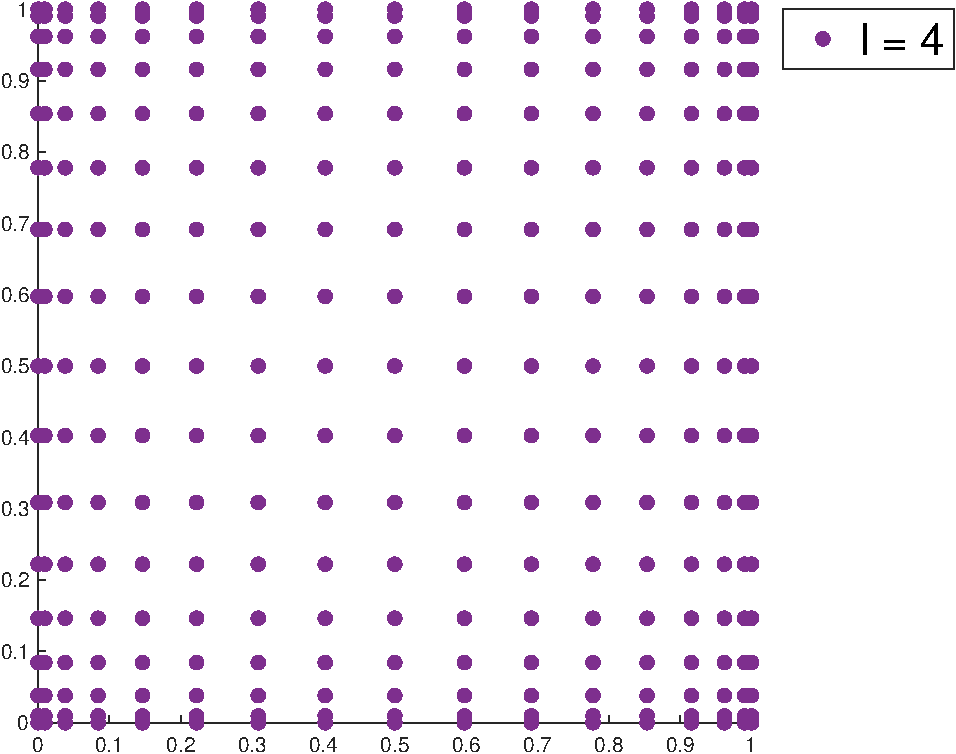
\includegraphics[width=0.27\linewidth]{full_grid_2d}
%             %         &
%             %         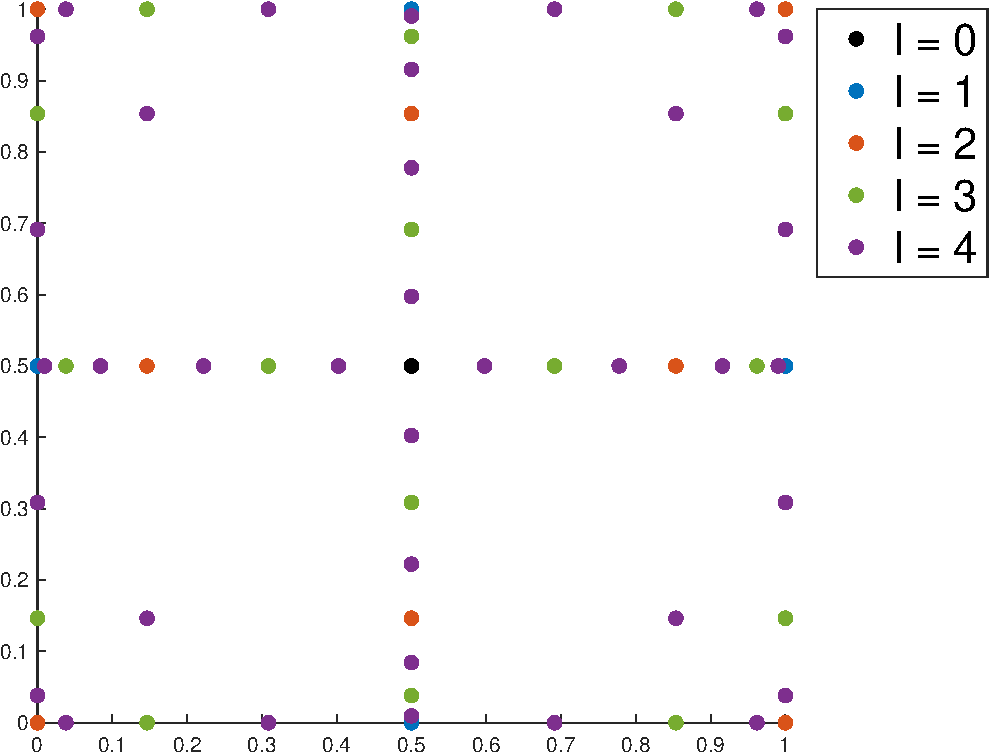
\includegraphics[width=0.27\linewidth]{sparse_grid_2d}
%             %         &
%             %         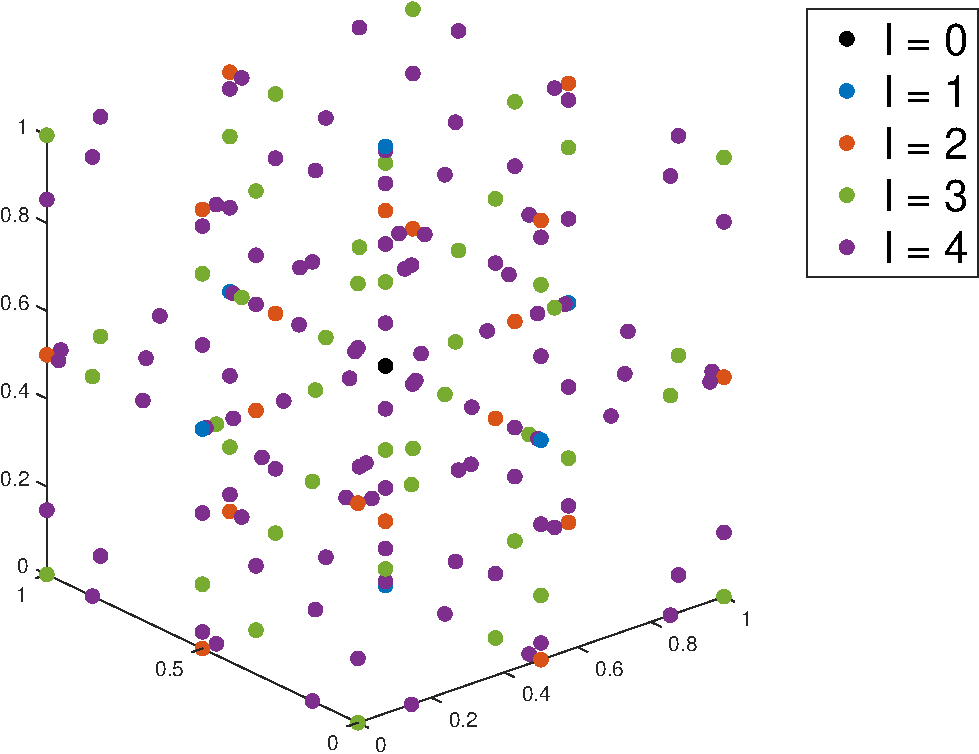
\includegraphics[width=0.27\linewidth]{sparse_grid_3d}
%             %     \end{tabular}
%             %     \caption*{{\footnotesize Left to right: Full tensor grid 2d, level 4. Chebyshev sparse grids for 2d and 3d from level 0 to level 4. \par}}
%             % \end{figure}

            
%             % \vspace{-10mm}
%             % \item[$\triangleright$] Compared to full tensor grid, {\bf Sparse Grid Stochastic Collocation} requires {\bf fewer grids} but with {\bf satisfying accuracy}.
%         \end{itemize} 
%     }
% \end{frame}





% %------------------------------------------------------------
% \begin{frame}[t]
%     \frametitle{Numerical Results}

%     {\footnotesize
%     \begin{itemize}[leftmargin=5pt] 
%             \item[$\triangleright$] {\bf Software:} {\footnotesize \textsc{Python} {\tt Chaospy}  toolbox -- J. Feinberg, \& H. Langtangen.}

%         Analyzing uncertainty using advanced Monte Carlo simulation and non-intrusive polynomial chaos expansions
        
%         \vspace{1mm}
%         {\fontsize{8}{8}\selectfont \textcolor{mygray2}{Chaospy: an open source tool for designing methods of uncertainty quantification. Journal of Computational Science, 11(2015).}
%         \par}
        
%         \item[$\triangleright$] Introduce two non-intrusive methods: {\bf Pseudo-spectral projection} \& {\bf point collocation}.
        
%         % \item[$\triangleright$] {\bf Pseudo-spectral projection:} apply a numerical integration scheme to estimate Fourier coefficients.

%         % Pros:  we can use sparse grid stochastic collocation to approximate the mean.
            
%         % \item[$\triangleright$] {\bf Point collocation:} collocation nodes can be arbitrary.

                
%         \item[$\triangleright$] Cons of this toolbox:

%         It does not allow secondary uncertainty analysis through MC simulation to yield more statistical metrics.
            
        
        
%     \end{itemize}
%     }
% \end{frame}

%------------------------------------------------------------
\begin{frame}[t]
    \frametitle{Comparison between $\widehat \rho_{1,k}$ and $\rho_{1,k}$}

%
\begin{figure}[!b]\centering
\begin{tabular}{ccc}
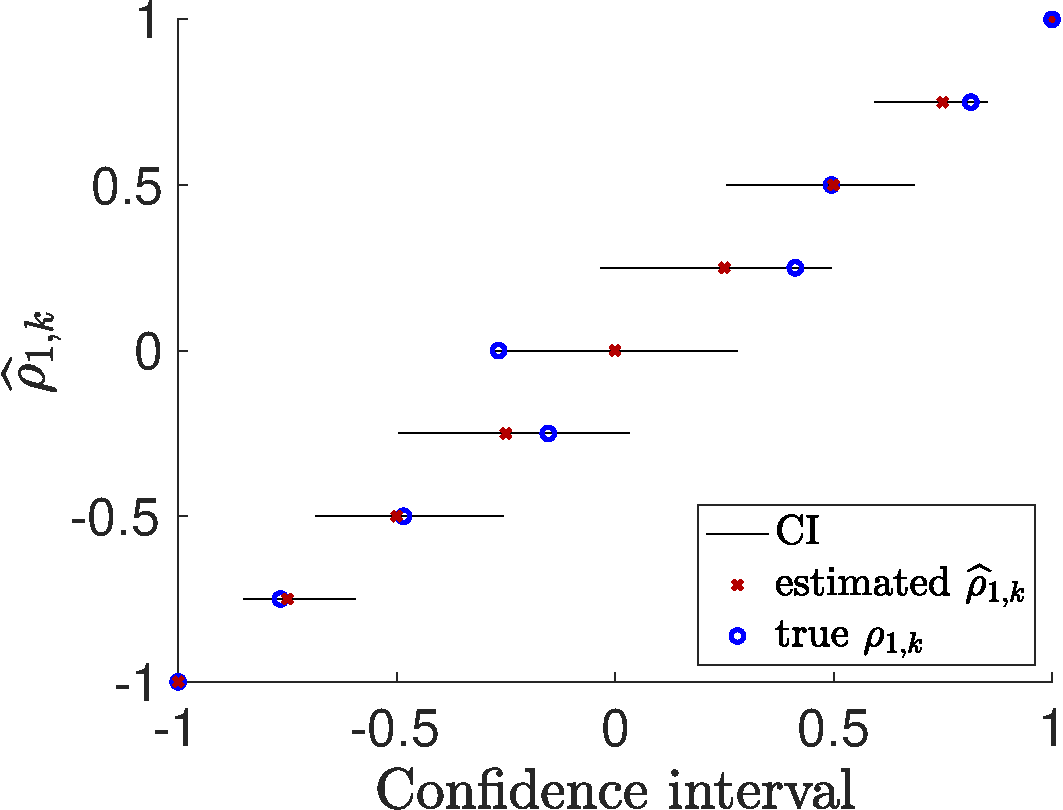
\includegraphics[width=0.3\linewidth]{./figures/Compare_true_estimate_rho.pdf}
\end{tabular}
% \caption{Comparison between $\widehat \rho_{1,k}$ and $\rho_{1,k}$.} 
\label{fig:CI_plot} 
\end{figure}
%
{\footnotesize
\begin{itemize}[leftmargin=5pt] 
    \item[$\circ$] Confidence intervals are generated  with pilot sample size $Q=10$ and $z_{\alpha/2}=1.96$ 
    \item[$\circ$] $\epsilon=10^{-2}$, $\sigma_1=10^{-1}$, 
    % \item[$\circ$] 
\end{itemize}
}


%
\begin{table}[ht]
\centering
\scalebox{0.4}{
\begin{tabular}{c|c|c|c|c|c|c|c|c|c|c|c|c|c|c|c|c|c|c|}
\hline
\multicolumn{1}{|c|}{ Cost per sample}&\multicolumn{2}{|c|}{ [100,          10,           1,        1000,         1,    1,           1,           1,         100]}\\
\hline
\hline
\multicolumn{1}{|c|}{} &true $\rho_{1,k}$&estimate $\widehat \rho_{1,k}$\\
\hline
\multicolumn{1}{|c|}{$\rho_{1,k}$} &[-1,  -0.650,  -0.464,  -0.402, -0.057,   0.038,   0.268,   0.836,  1]&[-1,-0.75,-0.5,-0.25,0,0.25,0.5,0.75,1]\\
% \multicolumn{1}{|c|}{} &-0.057   0.038   0.268   0.836  1&\\
\hline
\multicolumn{1}{|c|}{Model selection (model index)}&[1,8]&[1,2,3]\\
\hline
\multicolumn{1}{|c|}{Sample size before ceil}&[34.73,   528.74] &[58.75,   157.02,   444.11]\\
\hline
\multicolumn{1}{|c|}{Variance before ceil}&1e-4&1e-4\\
\hline
\multicolumn{1}{|c|}{Sampling cost before ceil}&4.00e+03 &7.89e+03\\
\hline
\hline
\multicolumn{1}{|c|}{Sample size after ceil}&[35,   529] &[59,   158,   445]\\
\hline
\multicolumn{1}{|c|}{Variance after ceil}&9.9331e-05&9.9549e-05\\
\hline
\multicolumn{1}{|c|}{Sampling cost after ceil}&4029 &7925\\
\hline
\end{tabular}
}
% \caption{}
\label{Tab:Offline_cost}
\end{table}
%

\end{frame}
%------------------------------------------------------------
%------------------------------------------------------------
\begin{frame}[t]
    \frametitle{Observation}
    {\footnotesize 
\begin{itemize}[leftmargin=5pt] 
     \item[$\triangleright$] {\bf Observation:} 
     \begin{itemize}[leftmargin=10pt] 
     \item [$\circ$] Sampling cost of $\widehat \rho_{1,k}$ is {\bf higher}  than that of $\rho_{1,k}$. This is due to the fact that different sets of models are selected and the difference between the true $\rho_{1,k}$ and the estimated $\widehat \rho_{1,k}$.
     \item [$\circ$] Overlap of confidence intervals, $\widehat \rho_{1,k}$ has monotonic trend, whereas the true $\rho_{1,k}$ does not have this behavior. This mismatch influences model selection and cost estimation.
        \item [$\circ$]The variance constraint is satisfied exactly when using real-valued sample sizes. When rounding up to the nearest integer, the resulting variance is slightly below the target tolerance.
        \item [$\circ$] Rounding sample sizes to integers has minimal effect on both variance and cost. In contrast, poor approximation of $\rho_{1,k}$ can lead to significant increases in sampling cost (e.g., from $\sim$4k to $\sim$8k).
     \end{itemize}
\end{itemize}
 }


\end{frame}
%------------------------------------------------------------

%------------------------------------------------------------
\begin{frame}[t]
    \frametitle{Comparison between $\widehat \rho_{1,k}$ and $\rho_{1,k}$}

%
\begin{figure}[!b]\centering
\begin{tabular}{ccc}
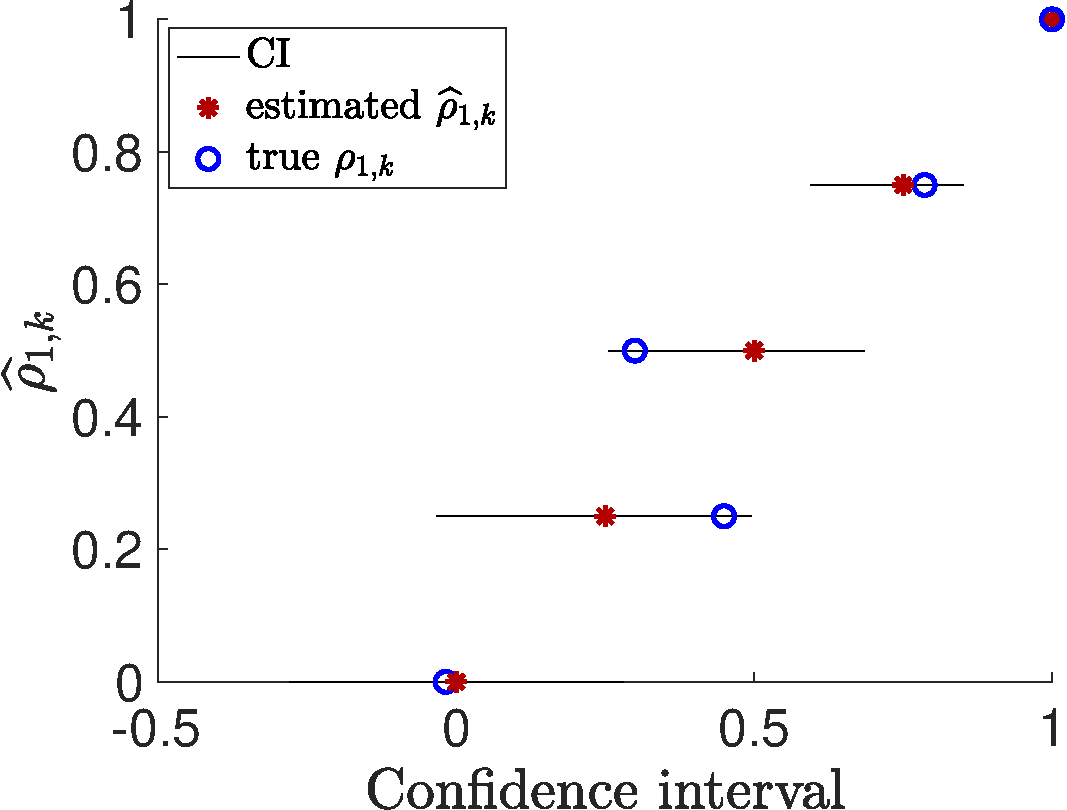
\includegraphics[width=0.3\linewidth]{./figures/Compare_true_estimate_rho_2.pdf}
\end{tabular}
% \caption{Comparison between $\widehat \rho_{1,k}$ and $\rho_{1,k}$.} 
\label{fig:CI_plot} 
\end{figure}
%
% {\footnotesize
% \begin{itemize}[leftmargin=5pt] 
%     \item[$\circ$] Confidence intervals are generated  with pilot sample size $Q=10$ and $z_{\alpha/2}=1.96$ 
%     \item[$\circ$] $\epsilon=10^{-2}$, $\sigma_1=10^{-1}$, 
%     % \item[$\circ$] 
% \end{itemize}
% }


%
\begin{table}[ht]
\centering
\scalebox{0.4}{
\begin{tabular}{c|c|c|c|c|c|c|c|c|c|c|c|c|c|c|c|c|c|c|}
\hline
\multicolumn{1}{|c|}{ Cost per sample}&\multicolumn{2}{|c|}{ [10,           1,           1,        1000,         100]}\\
\hline
\hline
\multicolumn{1}{|c|}{} &true $\rho_{1,k}$&estimate $\widehat \rho_{1,k}$\\
\hline
\multicolumn{1}{|c|}{$\rho_{1,k}$} &[-1.7700e-02,   4.4940e-01,   2.9981e-01,   7.8605e-01,   1]&[0,0.25,0.5,0.75,1]\\
% \multicolumn{1}{|c|}{} &-0.057   0.038   0.268   0.836  1&\\
\hline
\multicolumn{1}{|c|}{Model selection (model index)}&[5,3]&[5,2]\\
\hline
\multicolumn{1}{|c|}{Sample size before ceil}&[83.82,   421.66] &[79.33,   458.01]\\
\hline
\multicolumn{1}{|c|}{Variance before ceil}&1e-4&1e-4\\
\hline
\multicolumn{1}{|c|}{Sampling cost before ceil}&8.8035e+03 &8.3910e+03\\
\hline
\hline
\multicolumn{1}{|c|}{Sample size after ceil}&[84,   422] &[80,   459]\\
\hline
\multicolumn{1}{|c|}{Variance after ceil}&9.9790e-05&9.9197e-05\\
\hline
\multicolumn{1}{|c|}{Sampling cost after ceil}& 8822&8459\\
\hline
\end{tabular}
}
% \caption{}
\label{Tab:Offline_cost}
\end{table}
%
{\footnotesize 
\begin{itemize}[leftmargin=5pt] 
     \item[$\triangleright$] {\bf Observation:} 
     \begin{itemize}[leftmargin=10pt] 
     \item [$\circ$] Sampling cost of $\widehat \rho_{1,k}$ is {\bf smaller} than that of $\rho_{1,k}$. Different models are selected.
     % \item [$\circ$] 
     \end{itemize}
\end{itemize}
 }
\end{frame}
%------------------------------------------------------------

%------------------------------------------------------------
\begin{frame}[t]
    \frametitle{Comparison between $\widehat \rho_{1,k}$ and $\rho_{1,k}$}
%
\begin{figure}[!b]\centering
\begin{tabular}{ccc}
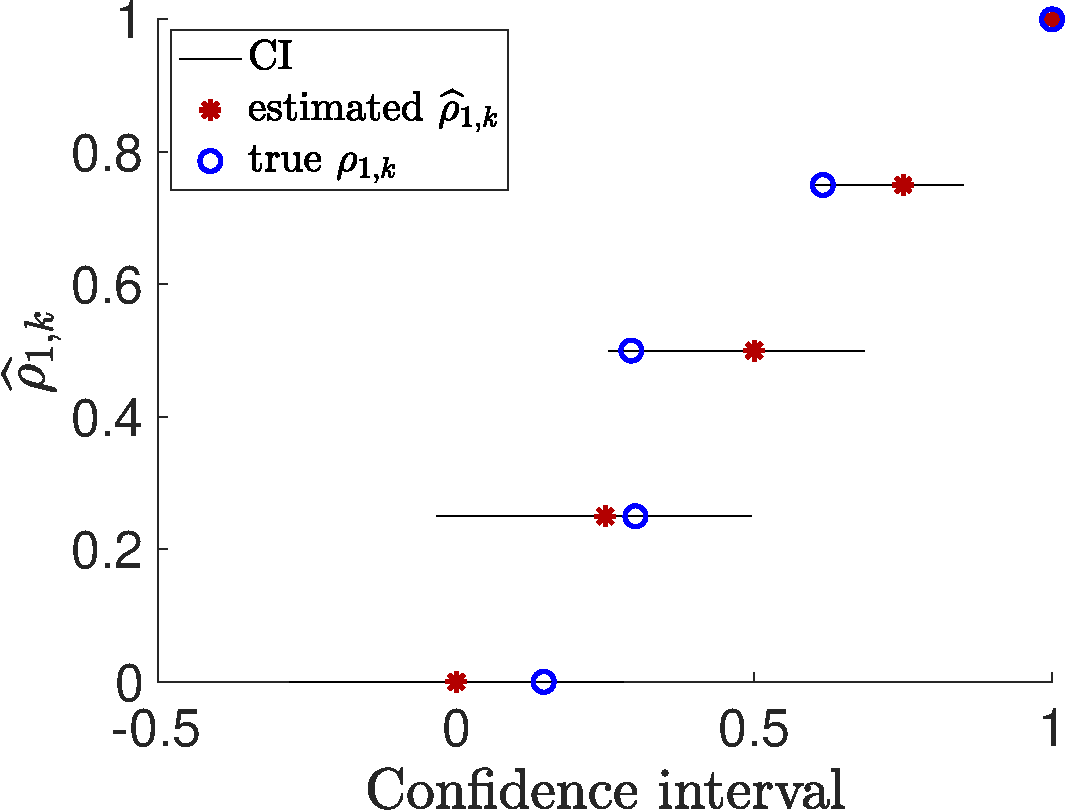
\includegraphics[width=0.3\linewidth]{./figures/Compare_true_estimate_rho_3.pdf}
\end{tabular}
% \caption{Comparison between $\widehat \rho_{1,k}$ and $\rho_{1,k}$.} 
\label{fig:CI_plot} 
\end{figure}
%
%
\begin{table}[ht]
\centering
\scalebox{0.4}{
\begin{tabular}{c|c|c|c|c|c|c|c|c|c|c|c|c|c|c|c|c|c|c|}
\hline
\multicolumn{1}{|c|}{ Cost per sample}&\multicolumn{2}{|c|}{ [10,           1,           1,        1000,         100]}\\
\hline
\hline
\multicolumn{1}{|c|}{} &true $\rho_{1,k}$&estimate $\widehat \rho_{1,k}$\\
\hline
\multicolumn{1}{|c|}{$\rho_{1,k}$} &[1.4674e-01,   3.0076e-01,   2.9375e-01,   6.1525e-01,   1]&[0,0.25,0.5,0.75,1]\\
% \multicolumn{1}{|c|}{} &-0.057   0.038   0.268   0.836  1&\\
\hline
\multicolumn{1}{|c|}{Model selection (model index)}&[5,4]&[5,4]\\
\hline
\multicolumn{1}{|c|}{Sample size before ceil}&[67.00,   522.88] &[48.71,   552.33]\\
\hline
\multicolumn{1}{|c|}{Variance before ceil}&1e-4&1e-4\\
\hline
\multicolumn{1}{|c|}{Sampling cost before ceil}&7.2226e+03 &5.4234e+03\\
\hline
\hline
\multicolumn{1}{|c|}{Sample size after ceil}&[67,   523] &[49,   553]\\
\hline
\multicolumn{1}{|c|}{Variance after ceil}&9.9994e-05&9.9458e-05\\
\hline
\multicolumn{1}{|c|}{Sampling cost after ceil}&7223&5453\\
\hline
\end{tabular}
}
% \caption{}
\label{Tab:Offline_cost}
\end{table}
%
%
{\footnotesize 
\begin{itemize}[leftmargin=5pt] 
     \item[$\triangleright$] {\bf Observation:} 
     \begin{itemize}[leftmargin=10pt] 
     \item [$\circ$] Sampling cost of $\widehat \rho_{1,k}$ is {\bf smaller} than that of $\rho_{1,k}$, even though same models are selected, the difference is due to the discrepancy in correlation coefficients.
     % \item [$\circ$] 
     \end{itemize}
\end{itemize}
 }
\end{frame}
%------------------------------------------------------------


% %------------------------------------------------------------
% \begin{frame}[t]
%     \frametitle{Numerical Results}

%     {\footnotesize
%     \begin{itemize}[leftmargin=5pt] 
%         % \item[$\triangleright$] Pseudo-spectral projection method--sparse grid
%         \item[$\triangleright$]  Parameter estimation:


        
        
%         \item[$\triangleright$] Quadrature nodes: Chebyshev Gauss-Lobatto nodes.
%             \item[$\triangleright$] Number of sparse grid nodes used: 61.

%             \begin{table}[ht]
%     	\centering
%     	\scalebox{0.8}{
%     		\begin{tabular}{c|c|c|c|c|c|c|c|c|c|c|}
%     			\cline{1-7}	
%     			\multicolumn{1}{|c|}{ Level $q$} &0&1&2&3&4&5\\
%     			\hline
%     			\multicolumn{1}{|c|}{\# of sparse grid nodes $P_q$}&\multicolumn{1}{c|}{1}&\multicolumn{1}{c|}{11}&\multicolumn{1}{c|}{61} &\multicolumn{1}{c|}{241} &\multicolumn{1}{c|}{801} &\multicolumn{1}{c|}{2433} \\
%     			% 			\hline
%     			% \multicolumn{1}{|c|}{ Time per realization (s.)} &0.13&0.38&1.59&8.65&44.64&210.27\\
%     			\hline
%     	\end{tabular}}
%     		% \caption{Mean running time, in seconds, of the direct solver on the uniformly refined mesh with increasing number of grid points based on 10 simulations. Level 2 mesh is the reference mesh.}
%     		% \label{Tab:CPUtime_CostEstimate}
%             \end{table}
%             % \item[$\triangleright$] Plot of functions $x_h^d(\cdot, \boldsymbol{\xi}_k)$ at sparse grid nodes $\boldsymbol{\xi}_k$ and expectation:
%             %     \begin{figure}[!t]\centering
%             %     \begin{tabular}{c}
%             %     \includegraphics[width=0.7\linewidth]{Surrog_l2_traj.pdf}
%             %     % \includegraphics[width=0.46\linewidth]{Altitude_vs_Time.pdf} &
%             %     % \includegraphics[width=0.46\linewidth]{Flight_Path_Angle_vs_Time.pdf} 
%             %     \end{tabular}
%             %     % \label{fig:CollectionPlot} 
%             %     \end{figure}

                
%             \item[$\triangleright$]
            
        
        
%     \end{itemize}
%     }
% \end{frame}


%------------------------------------------------------------
\begin{frame}[t]
    \frametitle{Numerical results}

\end{frame}
%------------------------------------------------------------






%-----------------------------------------------------------
\begin{frame}
% \frametitle{$|\!\!\sim\! \underline{\hspace{0.25cm}}\!\sim\!\! |@ \underline{\hspace{0.25cm}} @|\!* \!\underline{\hspace{0.25cm}}\!*\!|. \underline{\hspace{0.25cm}} .|- \underline{\hspace{0.25cm}} -|G \underline{\hspace{0.25cm}} G|x\underline{\hspace{0.25cm}} x|/\underline{\hspace{0.25cm}}\backslash|w_w|Q\underline{\hspace{0.25cm}}Q|>\underline{\hspace{0.25cm}}>|=\underline{\hspace{0.25cm}}=|+\underline{\hspace{0.25cm}}+|\#\underline{\hspace{0.25cm}}\#|z\underline{\hspace{0.25cm}}z|>\underline{\hspace{0.25cm}}<|6\underline{\hspace{0.25cm}}9|$}


	\begin{center}
	{\fontsize{35}{70}\selectfont  Thank You $|\neg\underline{\hspace{0.4cm}}\neg|$}
	\end{center}
\end{frame}
%----------------------------------------------------------------
\end{document}